
\documentclass{article}

\usepackage[utf8]{inputenc}

\usepackage[T1]{fontenc}

\usepackage{geometry}
\geometry{a4paper}

\usepackage{float}
\restylefloat{table}

\usepackage[english]{babel}

%\usepackage{setspace}
%\doublespacing

\usepackage{amsfonts}
\usepackage{amsmath}

% for lucid chart images
\usepackage{graphicx}

\begin{document}

\newpage

\section{Complexity as Bounded Rationality}

\subsection{Nash Equilibrium}
	
\noindent Let $G$ be a game with $K$ players. For each player $k$ we have
\begin{itemize}
	\item action set $A_k$ of actions available to $k$
	\item strategy set $\Delta(A_k)$ of distributions over the actions in $A_k$.
	\item payoff function $\mu_k: \Pi_{i=1}^K A_i \longrightarrow \mathbb{R}$
\end{itemize}

\noindent A Nash Equilibrium $S$ is a strategy assignment $(p_1,..., p_k)$ such that for each player $k$:
\begin{equation}
\forall q \in \Delta(A_k): \mu_k(p_k, S_{-k}) \ge \mu_k(q, S_{-k})
\end{equation}

\newpage

\subsection {Prisoner's Dilemma}

\begin{table}[H]
	\centering
	\caption{Prisoner's Dilemma}
	\label{pdpayoffs}
	\begin{tabular}{lll}
		& C                        & D                        \\ \cline{2-3} 
		\multicolumn{1}{l|}{C} & \multicolumn{1}{l|}{3,3} & \multicolumn{1}{l|}{0,4} \\ \cline{2-3} 
		\multicolumn{1}{l|}{D} & \multicolumn{1}{l|}{4,0} & \multicolumn{1}{l|}{1,1} \\ \cline{2-3} 
	\end{tabular}
\end{table}

\begin{itemize}
	\item Consider the $n$-round prisoners dilemma.
	\item The action set $A_n$ for each player is now of the form $\Pi_{i=1}^n A$, where $A = \lbrace C,D \rbrace $, and so $|A_n| = 2^n$.
	\item if $n =1$, the only Nash equilibrium is $(D,D)$
	\item if $1 < n < +\infty$, using backwards induction shows the only Nash equilbrium is $(D^n, D^n)$
\end{itemize}

\subsection{Questions}

\noindent Question: how can we quantify the complexity of strategies?\\\\
\noindent Question: is it reasonable to assume that players will use far more complex strategies in lieu of simpler ones to achiev\textsl{}e marginally greater payoffs?

\newpage

\subsection{Bounded Rationality}

The complexity of a strategy can be quantified by the number of states required by a finite automaton which implements the strategy, e.g.:

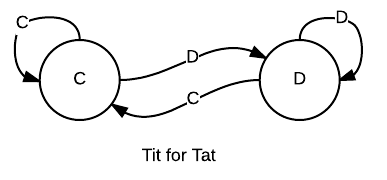
\includegraphics[scale=0.5]{tit4tat}

\noindent restrict the complexity of strategies $\implies$ restrict the number of states in the automata\\\textsl{\textsl{}}

\noindent For instance: an automata with less than $n$ states cannot count up to $n$ and so our backwards induction argument would no longer be valid

\end{document}